\documentclass[a4paper,12pt]{article}
\usepackage[top = 2.5cm, bottom = 2.5cm, left = 2.5cm, right = 2.5cm]{geometry}
% Unfortunately, LaTeX has a hard time interpreting German Umlaute. The following two lines and packages should help. If it doesn't work for you please let me know.
\usepackage[T1]{fontenc}
\usepackage[utf8]{inputenc}
% The following two packages - multirow and booktabs - are needed to create nice looking tables.
\usepackage{multirow} % Multirow is for tables with multiple rows within one cell.
\usepackage{booktabs} % For even nicer tables.
% As we usually want to include some plots (.pdf files) we need a package for that.
\usepackage{graphicx}
% The default setting of LaTeX is to indent new paragraphs. This is useful for articles. But not really nice for homework problem sets. The following command sets the indent to 0.
\usepackage[spanish]{babel}
\usepackage{setspace}
\setlength{\parindent}{0in}
% Package to place figures where you want them.
\usepackage{float}
% The fancyhdr package let's us create nice headers.
\usepackage{fancyhdr}
\usepackage{amsmath}
\usepackage{amssymb}
\usepackage{natbib}
\usepackage{graphicx}
\usepackage{subcaption}
\usepackage{booktabs}
\usepackage{etoolbox}
\usepackage{amsthm}
\newenvironment{solution}
  {\renewcommand\qedsymbol{$\blacksquare$}\begin{proof}[Solución]}
  {\end{proof}}
\pagestyle{fancy}

\fancyhf{}

\lhead{\footnotesize Hoja de trabajo 1}
\rhead{\footnotesize  Rompich}
\cfoot{\footnotesize \thepage}



\begin{document}
    \thispagestyle{empty} % This command disables the header on the first page.

    \begin{tabular}{p{15.5cm}} % This is a simple tabular environment to align your text nicely
    \begin{tabbing}
    Universidad del Valle de Guatemala \\ 5 de febrero de 2021  \\
    Rudik R. Rompich   - Carné: 19857\\
    \end{tabbing}
    Estadística 2 - Eugenio Aristondo \\
    \hline % \hline produces horizontal lines.
    \\
    \end{tabular} % Our tabular environment ends here.
    \vspace*{0.3cm} % Now we want to add some vertical space in between the line and our title.
    \begin{center} % Everything within the center environment is centered.
    {\Large \bf Hoja de trabajo 1 
} % <---- Don't forget to put in the right number
        \vspace{2mm}
    \end{center}
    \vspace{0.4cm}


La resistencia a la tensión de cierto elemento estructural es una característica importante. La tabla siguiente da información de la resistencia a la tensión (y), el espesor de la soldadura (x1), la altura del poste (x2), el grosor del elemento (x3), la longitud del elemento (x4), el ancho de la unión (x5) y el ancho del poste (x6).

\section{I}
Elabore la matriz de correlación para este conjunto de datos y elija como regresores preliminares aquellos cuya correlación con los demás es menor o igual a |0.30|.
\begin{center}
     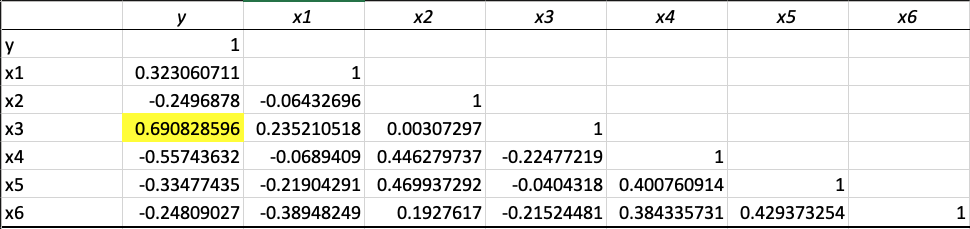
\includegraphics[scale=0.4]{matrix.png}
\end{center}


\section{II. RLS}
a) Encuentre el mejor modelo de regresión lineal simple. Y verifique los supuestos.
\begin{center}
     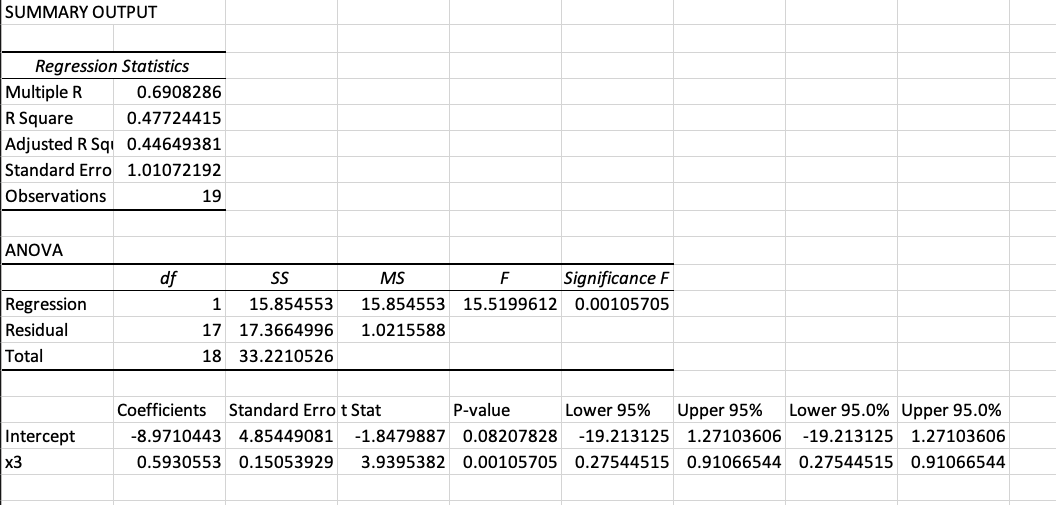
\includegraphics[scale=0.4]{model1.png}
\end{center}
\begin{align}
    \intertext{Lo que implica que el mejor modelo de regresión lineal simple es:}
    y= 0.593055296x_3-8.971044274 
\end{align}
Por otra parte, los supuestos: 
\begin{itemize}
    \item Linealidad: Según el $R^2$ es de 0.47724415, lo que implica que es un modelo con deficiencias y no tan preciso. El supuesto, sin embargom, se cumple.
    
     \begin{center}
        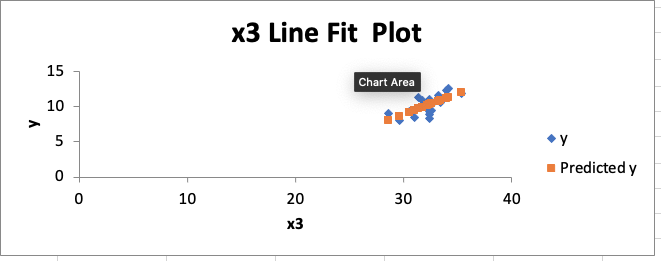
\includegraphics[scale=0.5]{fit.png}
    \end{center}
    \item Homocedasticidad: La variación de residuos es el mismo para cada valor de X.\newline\newline 
    Como se observa en el análisis de residuos, parece indicar que casi todos los puntos cumplen el supuesto, aunque el residuo de 10.5 indica una leve diferencia en este supuesto.
    \begin{center}
     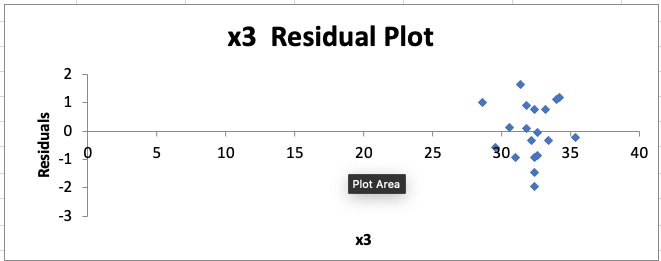
\includegraphics[scale=0.4]{homo.png}
    \end{center}
    \item Independencia: Las observaciones son independientes de cada una.\newline\newline 
    
    Como se observa en el análisis de independencia, el supuesto parece cumplirse.
    
    \begin{center}
     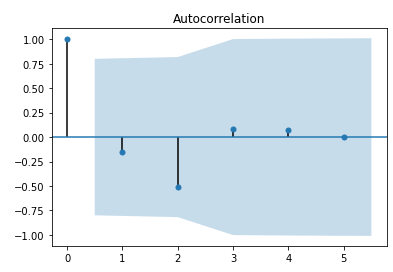
\includegraphics[scale=0.4]{inde.png}
    \end{center}
    
    \item Normalidad: Por cada valor arreglado de X, Y es normalmente distribuida. \newline\newline 
    
    Es una distribución normal con una leve variación. 
    \begin{center}
        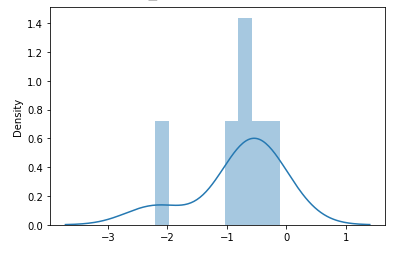
\includegraphics[scale=0.5]{norm1.png}
    \end{center}
    El análisis de promedios parece mostrar que el supuesto es correcto.
    \begin{center}
        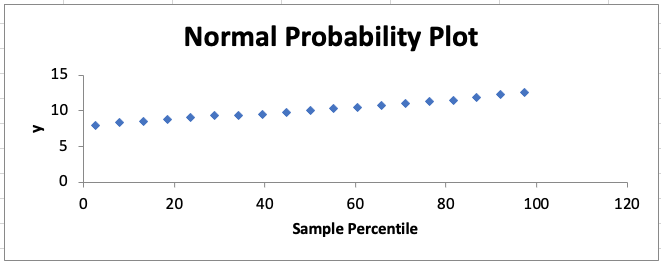
\includegraphics[scale=0.5]{norm2.png}
    \end{center}
\end{itemize}
\section{III. RLM}
b) Haga el análisis completo de regresión lineal múltiple mediante la eliminación en reversa tomando en cuenta todos los regresores y las interacciones dobles solamente de aquellos regresores cuya correlación excede el |0.30|\newline\newline
 \begin{center}
        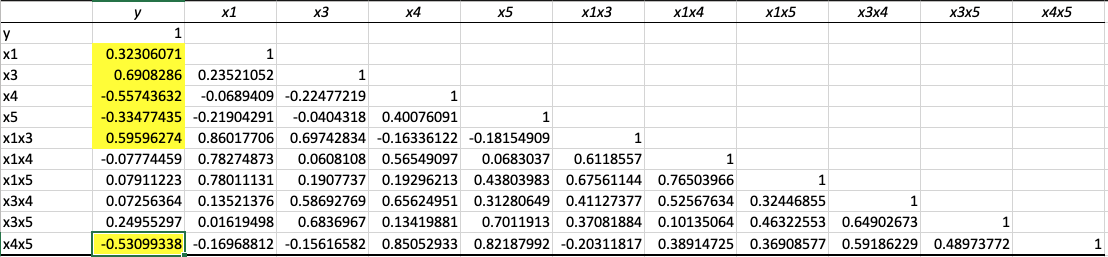
\includegraphics[scale=0.4]{model2.png}
\end{center}
c) Plantee el modelo final.\newline\newline
 \begin{center}
        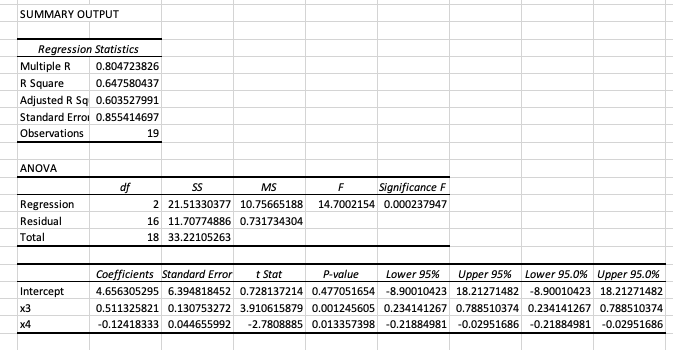
\includegraphics[scale=0.5]{modelo_multi.png}
\end{center}

d) Plantee la ecuación ajustada.\newline\newline
$$y=0,511325821x_3-0,1241833x_2 +4,656305295$$
e) Haga análisis completo de residuos. \newline\newline

Análisis de residuos de la variable $x_3$
 \begin{center}
        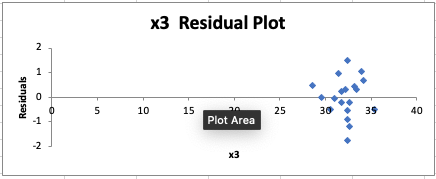
\includegraphics[scale=0.5]{res1.png}
\end{center}
Análisis de residuos de la variable $x_4$
\begin{center}
        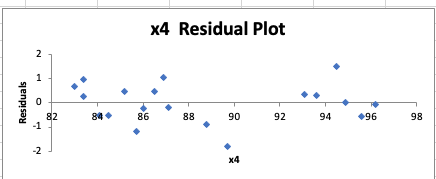
\includegraphics[scale=0.5]{res2.png}
\end{center}



\end{document}